\documentclass{article}
\usepackage{graphicx} % Required for inserting images

\usepackage[english, russian]{babel}
\usepackage[T2A]{fontenc}			% кодировка
\usepackage[utf8]{inputenc}			% кодировка исходного текста

\title{\textbf{Лабораторная работа 1.1.4.} \linebreak
ИЗУЧЕНИЕ СТАТИСТИЧЕСКИХ ЗАКОНОМЕРНОСТЕЙ НА
ПРИМЕРЕ ИЗМЕРЕНИЯ ФОНА КОСМИЧЕСКОГО ИЗЛУЧЕНИЯ}
\author{Попова Софья Б04-401}
\date{September 2024}

\begin{document}

\maketitle

\section*{Цель работы}
Познакомиться с основными понятиями статистики; на примере статистики регистрации фоновых космических частиц изучить статистические закономерности однородного во времени случайного процесса; проверить возможность описания исследуемого процесса статистическими законами Пуассона и Гаусса; измерить среднее число регистрируемых космических лучей в секунду и определить
погрешность результата.

\section*{Оборудование}
Счётчик Гейгера—Мюллера, компьютер с интерфейсом
для связи со счётчиком.

\section*{Теоретическая часть}
При любом физическом измерении результат, получаемый на опыте, несколько отличается от «истинного» значения измеряемой величины, поэтому бОльший смысл в себе несет средняя величина некоторого количества измерений, а не результат одного.

\noindent
(В этой работе будем считать, что все погрешности, кроме статистических, пренебрежимо малы и не учитываются.)

\noindent
Наиболее важной характеристикой является среднее число регистрируемых частиц в единицу времени. Если $n_1$, $n_2$, … $n_N$ — результаты $N$ проведённых в одинаковых условиях измерений, можно вычислить выборочное среднее значение числа измерений:
\begin{equation}\label{нср}
\overline{n}\equiv\frac{1}{N}\sum_{i=1}^{N} {n_i}
\end{equation} 
Выборочное среднее будет стремиться к некоторому конечному пределу, который
можно назвать «истинным» средним значением числа регистрируемых частиц:
\begin{equation}\label{нср}
\overline{n}=\lim{(n)}
\end{equation} 
Кроме среднего значения важно знать, насколько сильно флуктуируют
значения $n_i$ от опыта к опыту, или же среднеквадратичное отклонение:
\begin{equation}\label{нср}
\sigma^2_n\equiv\frac{1}{N}{\sum_{i}^{N} {(n_i-(n))^2}}
\end{equation}
Тогда погрешность среднего значения (n) при независимых измерениях связана со стандартным отклонением формулой:
\begin{equation}\label{нср}
\sigma_{(n)}=\frac{\sigma_{n}}{\sqrt[]{N}}
\end{equation}

\noindent
\textbf{Пуассоновский процесс}

\noindent
Если случайные события (регистрация частиц) однородны во времени
(не меняют своей средней интенсивности), а каждое последующее событие
никак не зависит от того, как и когда произошло предыдущее, то последовательность таких событий принято называть \textit{пуассоновским процессом}. 

\noindent
Вероятности $w_n$ того, что в эксперименте будет обнаружено $n$ частиц, для распределения Пуассона имеют вид:
\begin{equation}\label{нср}
w_n=\frac{\overline{n}^{n}}{n!}e^{-n}
\end{equation}
Для пуассоновского процесса справедливо равенство:
\begin{equation}\label{нср}
\sigma=\sqrt[]{\overline{n}}
\end{equation}
На практике можно ожидать приближенное равенство для выборочных значений:
\begin{equation}\label{нср}
\sigma_n\approx\sqrt[]{(n)}
\end{equation}

\noindent
\textbf{Погрешность эксперимпента}

\noindent
Еcли подставить св-во распределения Пуассона (6) в формулу (4), получится среднеквадратичная погрешность определения среднего:  
\begin{equation}\label{нср}
\sigma_{(n)}=\frac{\sigma_{n}}{\sqrt[]{N}}=\sqrt[]{\frac{(n)}{N}}
\end{equation}
Для относительного значения погрешности:
\begin{equation}\label{нср}
\varepsilon_{(n)}=\frac{\sigma_{(n)}}{(n)}={\frac{1}{\sqrt[]{(n)N}}} 
\end{equation} 
Отсюда, единственный способ увеличить точность опыта — увеличивать общее число регистрируемых частиц за счёт увеличения совокупного времени измерений.

\section*{Экспериментальная часть}
В ходе работы получено 4000 значений числа зарегестрированных частиц. Эти данные сгруппированы с различными интервалами: $\tau$=20с; $\tau$=40с; $\tau$=80с (таблицы 1, 3, 5). На их основе составлены таблицы 2, 4, 6, в которых содержатся данные для построения гистограмм.

\noindent
Вычислим среднее число регистрируемых частиц по формуле (1): 
$$\overline{n_{20}}\equiv\frac{1}{20}\sum_{i=1}^{20} {n_i}\approx24,17$$
$$\overline{n_{40}}\equiv\frac{1}{40}\sum_{i=1}^{40} {n_i}\approx49,67$$
$$\overline{n_{80}}\equiv\frac{1}{80}\sum_{i=1}^{80} {n_i}\approx100,54$$
среднеквадратичное отклонение по формуле (3):
$$\sigma_{n_{20}}\equiv\sqrt[]{\frac{1}{20}\sum_{i}^{N} {(n_i-\overline{n_{20}})^2}}\approx15,53$$
$$\sigma_{n_{40}}\equiv\sqrt[]{\frac{1}{40}\sum_{i}^{N} {(n_i-\overline{n_{40}})^2}}\approx11,55$$
$$\sigma_{n_{80}}\equiv\sqrt[]{\frac{1}{80}\sum_{i}^{N} {(n_i-\overline{n_{80}})^2}}\approx7,89$$
погрешность среднего значения по формуле (4):
$$\sigma_{n_{20}}=\frac{\sigma_{n_{20}}}{\sqrt[]{N}}=\frac{15,53}{\sqrt[]{20}}\approx3,47$$
$$\sigma_{n_{40}}=\frac{\sigma_{n_{40}}}{\sqrt[]{N}}=\frac{11,55}{\sqrt[]{40}}\approx1,83$$
$$\sigma_{n_{80}}=\frac{\sigma_{n_{80}}}{\sqrt[]{N}}=\frac{7,89}{\sqrt[]{80}}\approx0,88$$
и сред. интенсивность регистрируемых частиц в сек по формуле $j=\frac{(n)}{\tau}$:
$$j_{n_{20}}=\frac{\overline{n_{20}}}{\tau}=\frac{24,17}{20}\approx1,21$$
$$j_{n_{40}}=\frac{\overline{n_{40}}}{\tau}=\frac{49,67}{40}\approx1,24$$
$$j_{n_{80}}=\frac{\overline{n_{80}}}{\tau}=\frac{100,54}{80}\approx1,26$$
Заметим, что средняя интенсивность регистрируемых частиц в секунду не зависит от величины интервала $\tau$ и числа точек N

\noindent
Для сравнения полученнных экспериментально данных с теоретическими, наложим поверх гистограммы для $\tau$=20с нормальное распределение Гаусса. Заметим, что гистограмма с достаточной точностью согласуется с распределением Гаусса.

\section*{Вывод}
Получены случайно изменяющиеся со временем данные об интенсивности потока космических частиц. Применены методы обработки данных для изучения статистических закономерностей при измерении интенсивности радиационного фона.


\newpage


\section*{Таблицы и графики}

\begin{table}[!h]
    \centering
    \begin{tabular}{|c|c|c|c|c|c|c|c|c|c|c|}
        \hline
         №опыта & 1 & 2 & 3 & 4 & 5 & 6 & 7 & 8 & 9 & 10 \\
         \hline
         0 & 26 & 23 & 22 & 29 & 29 & 19 & 27 & 25 & 28 & 25 \\
        10 & 24 & 26 & 25 & 26 & 33 & 28 & 20 & 18 & 29 & 28 \\
        20 & 21 & 25 & 24 & 27 & 18 & 15 & 25 & 21 & 18 & 26 \\
        30 & 28 & 30 & 23 & 22 & 26 & 20 & 26 & 23 & 23 & 33 \\
        40 & 24 & 23 & 20 & 30 & 16 & 27 & 20 & 21 & 27 & 27 \\
        50 & 17 & 19 & 21 & 24 & 21 & 15 & 31 & 27 & 28 & 23 \\
        60 & 27 & 25 & 31 & 17 & 27 & 27 & 24 & 16 & 24 & 15 \\
        70 & 32 & 25 & 22 & 19 & 19 & 31 & 24 & 22 & 27 & 26 \\
        80 & 25 & 25 & 21 & 36 & 30 & 26 & 23 & 19 & 32 & 24 \\
        90 & 21 & 24 & 23 & 27 & 17 & 26 & 11 & 23 & 19 & 19 \\
        100 & 23 & 15 & 22 & 39 & 20 & 17 & 17 & 19 & 30 & 28 \\
        110 & 26 & 24 & 17 & 32 & 23 & 21 & 24 & 12 & 29 & 28 \\
        120 & 24 & 32 & 21 & 19 & 21 & 22 & 25 & 20 & 23 & 29 \\
        130 & 21 & 21 & 31 & 34 & 30 & 27 & 14 & 28 & 27 & 34 \\
        140 & 25 & 23 & 29 & 22 & 27 & 10 & 25 & 27 & 14 & 24 \\
        150 & 23 & 32 & 30 & 25 & 21 & 25 & 29 & 25 & 21 & 26 \\
        160 & 31 & 21 & 28 & 31 & 18 & 22 & 22 & 23 & 19 & 27 \\
        170 & 25 & 16 & 23 & 21 & 25 & 21 & 20 & 22 & 29 & 24 \\
        180 & 30 & 24 & 19 & 32 & 17 & 23 & 27 & 32 & 22 & 24 \\
        190 & 29 & 29 & 29 & 18 & 23 & 25 & 27 & 31 & 24 & 32 \\
        \hline
    \end{tabular}
    \caption{Число срабатываний счетчика за 20 секунд}
\end{table}

\begin{table}[!h]
    \centering
    \begin{tabular}{|c|c|c|}
        \hline
         Число импульсов & Число случаев & Доля случаев \\
         \hline
        10 & 1 & 0,005 \\
        11 & 1 & 0,005 \\
        12 & 1 & 0,005 \\
        14 & 2 & 0,01 \\
        15 & 4 & 0,02 \\
        16 & 3 & 0,015 \\
        17 & 7 & 0,035 \\
        18 & 5 & 0,025 \\
        19 & 11 & 0,055 \\
        20 & 7 & 0,035 \\
        21 & 17 & 0,085 \\
        22 & 11 & 0,055 \\
        23 & 18 & 0,09 \\
        24 & 17 & 0,085 \\
        25 & 18 & 0,09 \\
        26 & 11 & 0,055 \\
        27 & 18 & 0,09 \\
        28 & 9 & 0,045 \\
        29 & 11 & 0,055 \\
        30 & 7 & 0,035 \\
        31 & 7 & 0,035 \\
        32 & 8 & 0,04 \\
        33 & 2 & 0,01 \\
        34 & 2 & 0,01 \\
        36 & 1 & 0,005 \\
        39 & 1 & 0,005 \\
        \hline
    \end{tabular}
    \caption{Данные для построения гистограммы для 20с}
\end{table}

\begin{table}[!h]
    \centering
    \begin{tabular}{|c|c|c|c|c|c|c|c|c|c|c|}
        \hline
         №опыта & 1 & 2 & 3 & 4 & 5 & 6 & 7 & 8 & 9 & 10 \\
         \hline
         0 & 49 & 53 & 50 & 53 & 54 & 51 & 52 & 61 & 40 & 57 \\
        10 & 47 & 53 & 34 & 46 & 47 & 60 & 46 & 47 & 53 & 56 \\
        20 & 48 & 52 & 44 & 41 & 55 & 37 & 47 & 37 & 62 & 51 \\
        30 & 52 & 48 & 55 & 42 & 42 & 58 & 42 & 52 & 47 & 53 \\
        40 & 50 & 58 & 57 & 43 & 57 & 47 & 52 & 44 & 36 & 39 \\
        50 & 38 & 65 & 37 & 40 & 62 & 50 & 49 & 45 & 37 & 58 \\
        60 & 58 & 41 & 46 & 45 & 53 & 43 & 67 & 59 & 46 & 63 \\
        70 & 51 & 52 & 40 & 54 & 39 & 55 & 55 & 48 & 55 & 47 \\
        80 & 56 & 60 & 40 & 45 & 48 & 42 & 46 & 47 & 44 & 55 \\
        90 & 57 & 51 & 41 & 60 & 46 & 58 & 49 & 50 & 59 & 58 \\
        \hline
    \end{tabular}
    \caption{Число срабатываний счетчика за 40 секунд}
\end{table}

\begin{table}[!h]
    \centering
    \begin{tabular}{|c|c|c|}
        \hline
         Число импульсов & Число случаев & Доля случаев \\
         \hline
        34 & 1 & 0,01 \\
        36 & 1 & 0,01 \\
        37 & 4 & 0,04 \\
        38 & 1 & 0,01 \\
        39 & 2 & 0,02 \\
        40 & 4 & 0,04 \\
        41 & 3 & 0,03 \\
        42 & 4 & 0,04 \\
        43 & 2 & 0,02 \\
        44 & 3 & 0,03 \\
        45 & 3 & 0,03 \\
        46 & 6 & 0,06 \\
        47 & 8 & 0,08 \\
        48 & 4 & 0,04 \\
        49 & 3 & 0,03 \\
        50 & 4 & 0,04 \\
        51 & 4 & 0,04 \\
        52 & 6 & 0,06 \\
        54 & 2 & 0,02 \\
        55 & 6 & 0,06 \\
        56 & 2 & 0,02 \\
        57 & 4 & 0,04 \\
        58 & 6 & 0,06 \\
        59 & 2 & 0,02 \\
        60 & 3 & 0,03 \\
        61 & 1 & 0,01 \\
        62 & 2 & 0,02 \\
        63 & 1 & 0,01 \\
        65 & 1 & 0,01 \\
        67 & 1 & 0,01 \\
        \hline
    \end{tabular}
    \caption{Данные для построения гистограммы для 40с}
\end{table}

\begin{table}[!h]
    \centering
    \begin{tabular}{|c|c|c|c|c|c|c|c|c|c|c|}
        \hline
         №опыта & 1 & 2 & 3 & 4 & 5 & 6 & 7 & 8 & 9 & 10 \\
         \hline
         0 & 103 & 104 & 106 & 113 & 98 & 100 & 80 & 109 & 93 & 110 \\
        10 & 102 & 88 & 92 & 85 & 113 & 101 & 98 & 101 & 95 & 101 \\
        20 & 111 & 101 & 107 & 97 & 76 & 105 & 78 & 116 & 94 & 97 \\
        30 & 100 & 93 & 100 & 126 & 110 & 105 & 94 & 94 & 104 & 102 \\
        40 & 117 & 86 & 92 & 94 & 101 & 108 & 102 & 106 & 102 & 117 \\
        \hline
    \end{tabular}
    \caption{Число срабатываний счетчика за 80 секунд}
\end{table}

\begin{table}[!h]
    \centering
    \begin{tabular}{|c|c|c|}
        \hline
         Число импульсов & Число случаев & Доля случаев \\
         \hline
        76 & 1 & 0,02 \\
        78 & 1 & 0,02 \\
        80 & 1 & 0,02 \\
        85 & 1 & 0,02 \\
        86 & 1 & 0,02 \\
        88 & 1 & 0,02 \\
        92 & 2 & 0,04 \\
        93 & 2 & 0,04 \\
        94 & 4 & 0,08 \\
        95 & 1 & 0,02 \\
        97 & 2 & 0,04 \\
        98 & 2 & 0,04 \\
        100 & 3 & 0,06 \\
        101 & 5 & 0,1 \\
        102 & 4 & 0,08 \\
        103 & 1 & 0,02 \\
        104 & 2 & 0,04 \\
        105 & 2 & 0,04 \\
        106 & 2 & 0,04 \\
        107 & 1 & 0,02 \\
        108 & 1 & 0,02 \\
        109 & 1 & 0,02 \\
        110 & 2 & 0,04 \\
        111 & 1 & 0,02 \\
        113 & 2 & 0,04 \\
        116 & 1 & 0,02 \\
        117 & 2 & 0,04 \\
        126 & 1 & 0,02 \\
        \hline
    \end{tabular}
    \caption{Данные для построения гистограммы для 80с}
\end{table}

\begin{figure}[t]
    \centering
    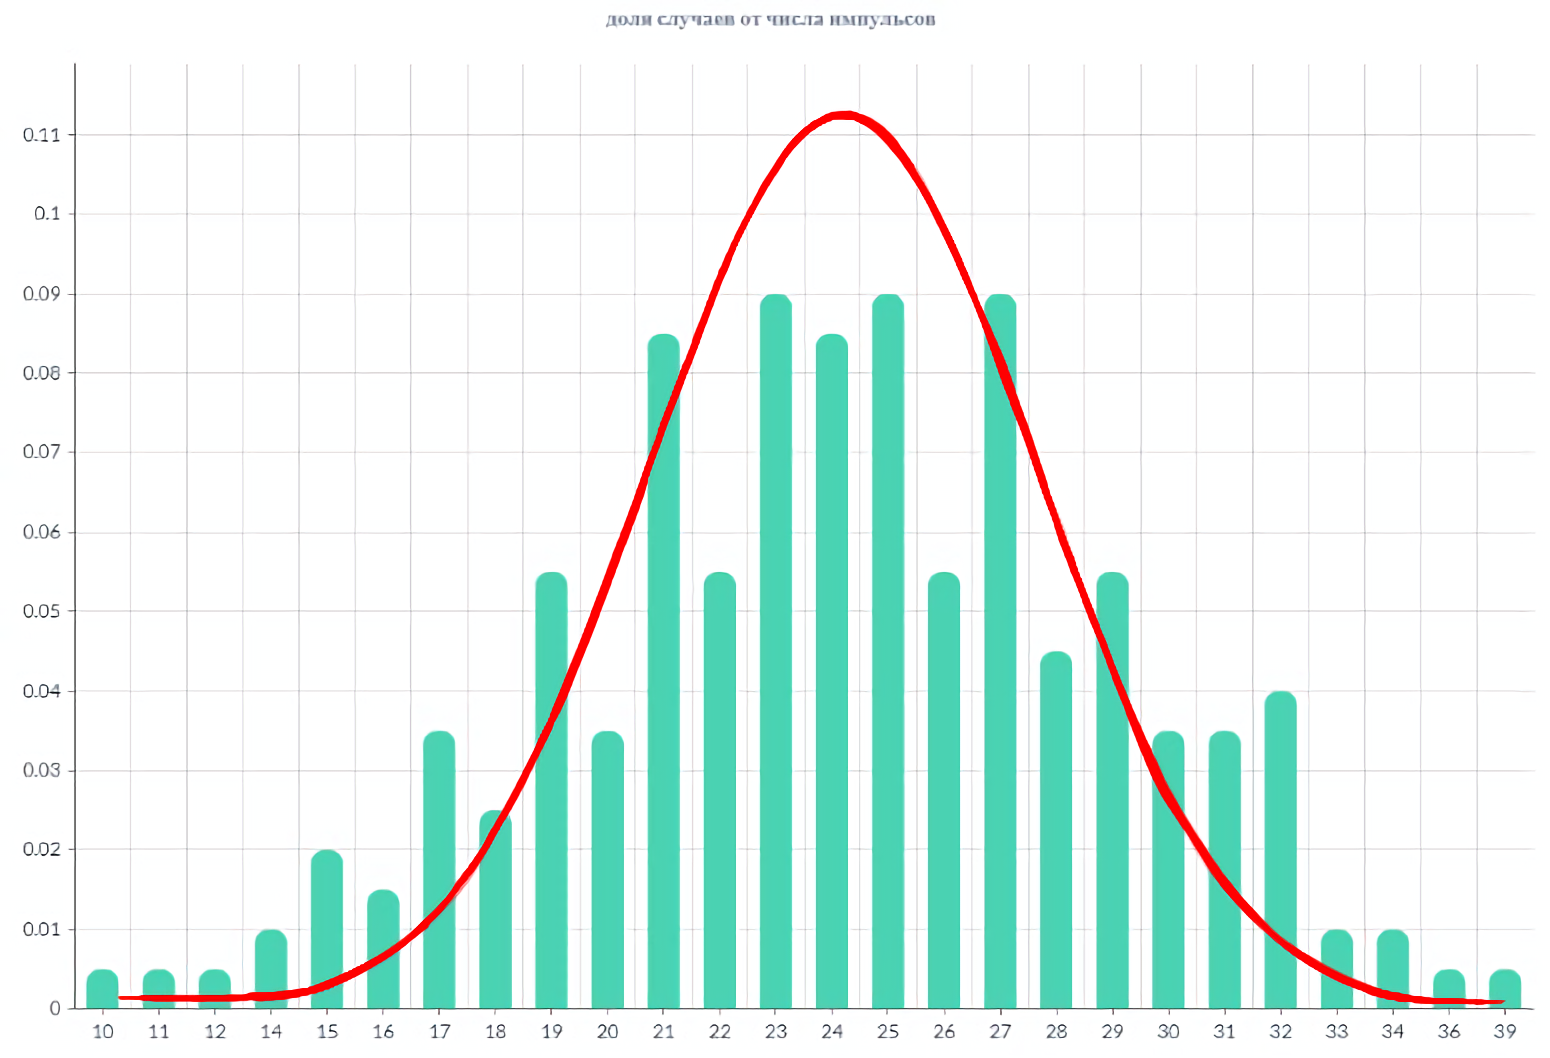
\includegraphics[width=0.65\linewidth]{Screenshot_4.png}
    \caption{Гистограмма распределения кол-ва частиц для 20с}
    \label{fig:enter-label}
\end{figure}

\begin{figure}[t]
    \centering
    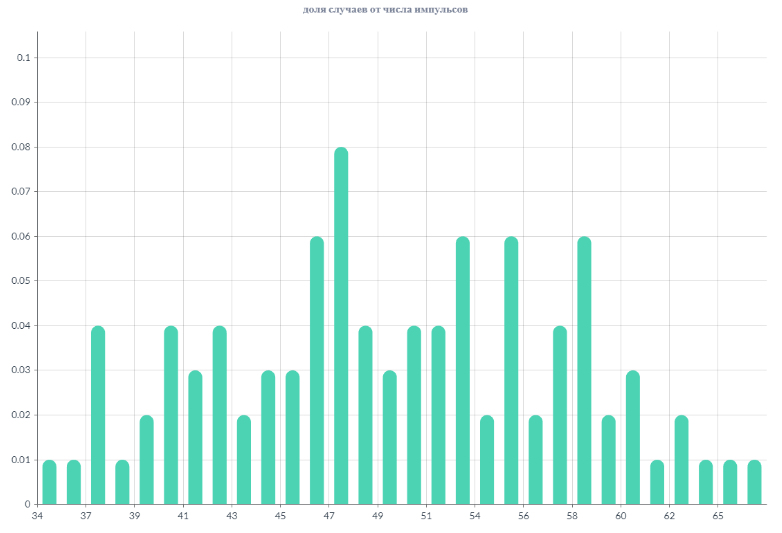
\includegraphics[width=0.65\linewidth]{Screenshot_2.png}
    \caption{Гистограмма распределения кол-ва частиц для 40с}
    \label{fig:enter-label}
\end{figure}

\begin{figure}[t]
    \centering
    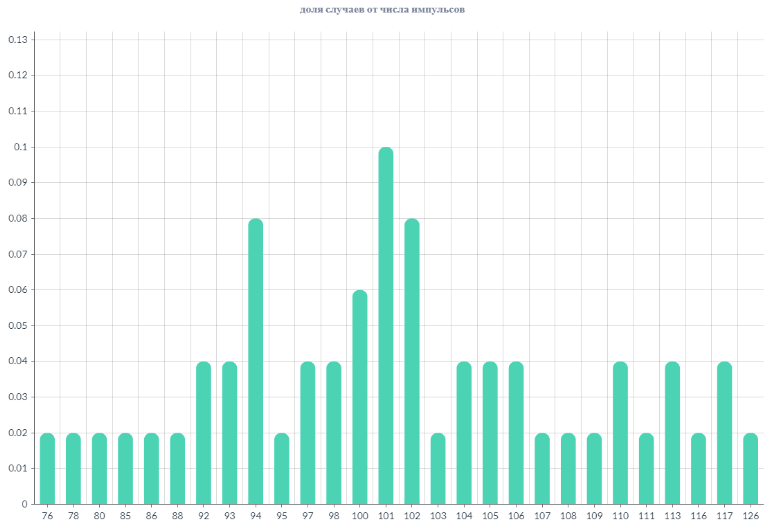
\includegraphics[width=0.65\linewidth]{Screenshot_1.png}
    \caption{Гистограмма распределения кол-ва частиц для 80с}
    \label{fig:enter-label}
\end{figure}

\end{document}
